\apendice{Plan de Proyecto Software}

\section{Introducción}

Sección en la que se va a desarrollar la planificación seguida en el proyecto, así como su viabilidad legal y económica.

Para llevar a cabo el seguimiento y planificación del proyecto se va a seguir la metodología \textit{Scrum} mediante Github, realizando un desarrollo incremental, dividido en sprints de una semana de duración cada uno. Durante cada sprint se irán creando y realizando las diferentes tareas correspondientes a los objetivos fijados en cada sprint. Al final de cada sprint se van a realizar las reuniones con los tutores para fijar las nuevas tareas de los nuevos sprints.

Para organizar las diferentes tareas se usará el tablero Kanban de Zenhub donde se mostrarán los diferentes estados de desarrollo en los que se encuentran las tareas.

El repositorio con el proyecto y las issues realizadas se puede encontrar en el siguiente enlace:
\url{https://github.com/AdrianAntonGarcia/-TFG-UBUSetas}

\section{Planificación temporal}

En esta sección se va a explicar la planificación del proyecto a través de los diferentes sprints realizados, explicando las fechas en las que se desarrollaron y que tareas se realizaron en cada uno. Los primeros cuatro sprint no se muestran de forma correcta debido a que no se cerraron las tareas de forma adecuada en esos sprint, este problema se arregló a partir del quinto sprint.

Cada sprint estará acompañado de su grafo Burndown y un listado de las tareas realizadas. El proyecto se inició el 11 de septiembre de 2017 y está planeado entregarse en el 14 de enero de 2018, planificando así su desarrollo en cuatro meses.

\subsection{Sprint 1}

Este sprint se desarrolló entre los días 11 y 17 de septiembre de 2017. Se realizaron las siguientes tareas y objetivos:

\begin{itemize}
	\item Estudiar las propuestas de los tutores para elegir como desarrollar el clasificador.
	\item Empezar a estudiar las herramientas disponibles para entrenar los modelos.
	\item Elegir una propuesta para crear el clasificador.
\end{itemize}

La primera semana del proyecto se dedicó a estudiar las diferentes técnicas propuestas para implementar el clasificador de imágenes, así como pensar las diferentes ventajas e inconvenientes de estas implementaciones y comprobar si eran viables con respecto al hardware y medios disponibles. Estas propuestas eran:
\begin{itemize}
	\item Crear un clasificador que se ejecute en un servidor y devuelva los resultados a la aplicación móvil. El modelo se puede reentrenar o entrenar desde cero.
	\item Reentrenar un modelo mediante la herramienta Tensorflow para poder ejecutar este modelo en el propio móvil.
\end{itemize}

\begin{figure}[h]
    \begin{center}%
        \begin{center}%
          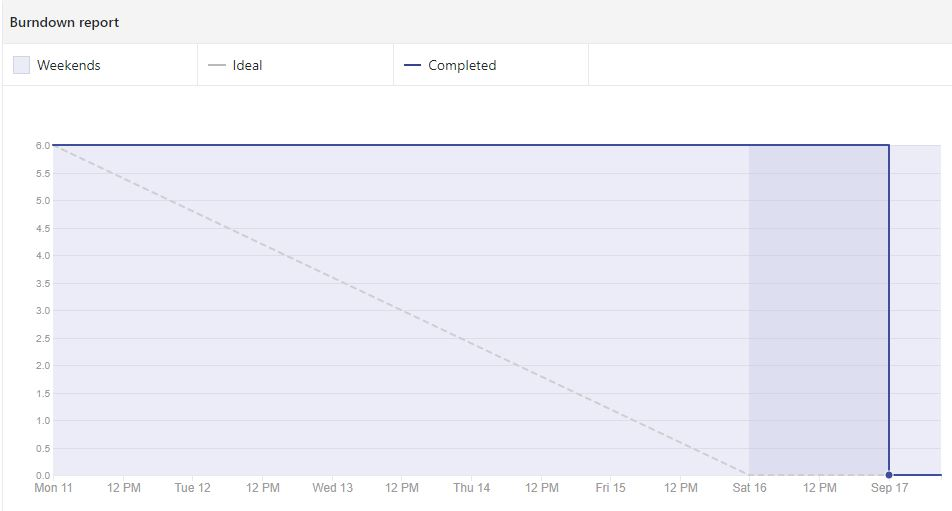
\includegraphics[width=1\textwidth]{imagenesAnexos/imagenesPlanificacion/sprint1}%
          \caption{Gráfico Burndown del sprint 1.}%
          \label{figSprint1}%
        \end{center}%
  	\end{center}%
\end{figure}%
\newpage

\subsection{Sprint 2}

Este sprint se desarrolló entre los días 18 y 24 de septiembre de 2017. Se realizaron las siguientes tareas y objetivos:

\begin{itemize}
	\item Estudiar las librerías de Tensorflow para el entrenamiento de los clasificadores.
	\item Estudiar los modelos Mobilenet e Inception.
	\item Estudiar como reentrenar los modelos mencionados.
	\item Estudiar como implementar los modelos en Android.
\end{itemize}

Esta semana relacionada con el segundo sprint se dedicó principalmente al estudio de las diferentes técnicas disponibles para entrenar modelos que pudieran funcionar en una arquitectura móvil. Para ello se realizó el estudio de las librerías de Tensorflow y se siguieron los ejemplos para reentrenamiento disponibles en el repositorio de Github público de Tensorflow. 

Además se estudiaron las capacidades Hardware de las que disponíamos para entrenar estos modelos, ya que son procesos que requieren bastante tiempo de ejecucción y había que comprobar si podíamos reentrenar con los equipos disponibles.

\begin{figure}[h]
    \begin{center}%
        \begin{center}%
          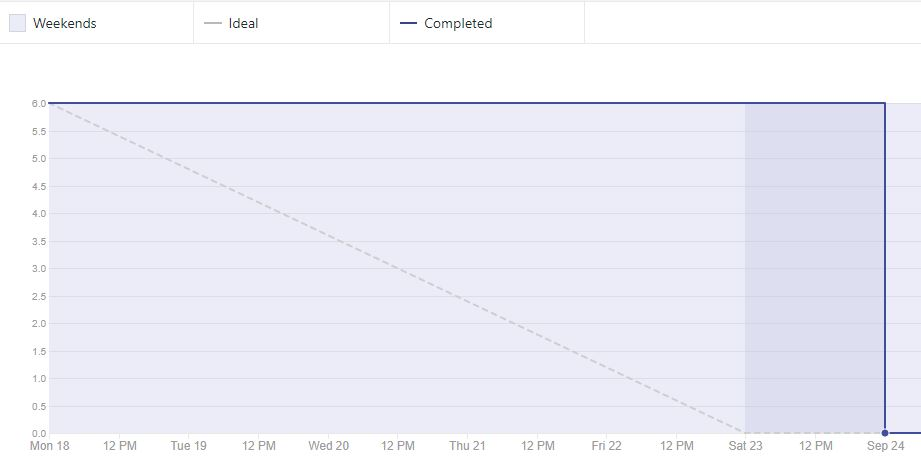
\includegraphics[width=1\textwidth]{imagenesAnexos/imagenesPlanificacion/sprint2}%
          \caption{Gráfico Burndown del sprint 2.}%
          \label{figSprint2}%
        \end{center}%
  	\end{center}%
\end{figure}%

\subsection{Sprint 3}

Este sprint se desarrolló entre el día 25 de septiembre y 1 de octubre de 2017. Se realizaron las siguientes tareas y objetivos:

\begin{itemize}
	\item Estudiar el entorno de programación Android Studio.
	\item Aprender a programar en Android.
	\item Implementar los modelos de clasificación en una aplicación Android.
\end{itemize}

El tercer sprint se dedicó principalmente a familiarizarme a desarrollar en Android. El objetivo era el de tener una base para poder ir implementando los modelos Mobilenet e Inception en una aplicación de prueba Android.

Tras esta semana se consiguió una primera demo que ejecutaba un modelo Mobilenet en el propio dispositivo móvil, aunque no funcionaba correctamente y tenía errores que se corrigieron según se fue profundizando en los diferentes aspectos a estudiar.

\begin{figure}[h]
    \begin{center}%
        \begin{center}%
          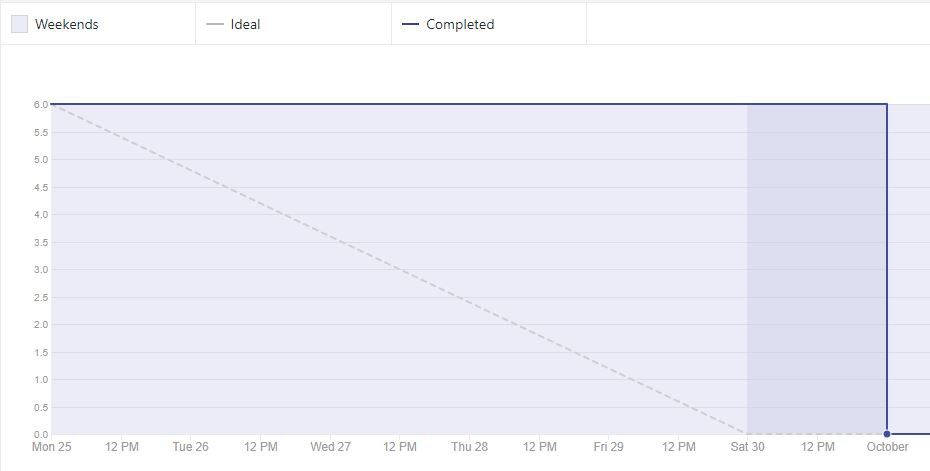
\includegraphics[width=1\textwidth]{imagenesAnexos/imagenesPlanificacion/sprint3}%
          \caption{Gráfico Burndown del sprint 3.}%
          \label{figSprint3}%
        \end{center}%
  	\end{center}%
\end{figure}%

\newpage

\subsection{Sprint 4}

Este sprint se desarrolló entre los días 2 y 8 de octubre de 2017. Se realizaron las siguientes tareas y objetivos:

\begin{itemize}
	\item Estudiar en qué consistía y cómo realizar consultas a una web semántica.
	\item Estudiar el marco de definición de recursos \textit{RDF}.
	\item Estudiar el lenguaje de consultas \textit{SPARQL}, para realizar las consultas a una web semántica.
	\item Estudiar el funcionamiento de la \textit{DBpedia} como Web semántica.
	\item Estudio de la herramienta \textit{Apache Jena} para realizar estas consultas a través de un programa Java.
	
\end{itemize}

Esta semana tenía como objetivo el entender en qué consistía una web semántica y cómo se podía implementar un programa Java que realizara consultas a una web semántica. El objetivo era el de estudiar como crear un programa Java que recopilara, de manera automática, información de las diferentes especies de setas.

Esta tarea tenía la complicación de que necesitábamos una web semántica que contuviera información de todas las setas, para poder facilitar la tarea de automatizar la extracción de información, y que esta se mostrará de manera uniforme. Tras estudiar las opciones disponibles se optó por la DBpedia ya que era la única que cumplía con las especificaciones necesarias y que contenía información suficiente de todas las especies.

\begin{figure}[h]
    \begin{center}%
        \begin{center}%
          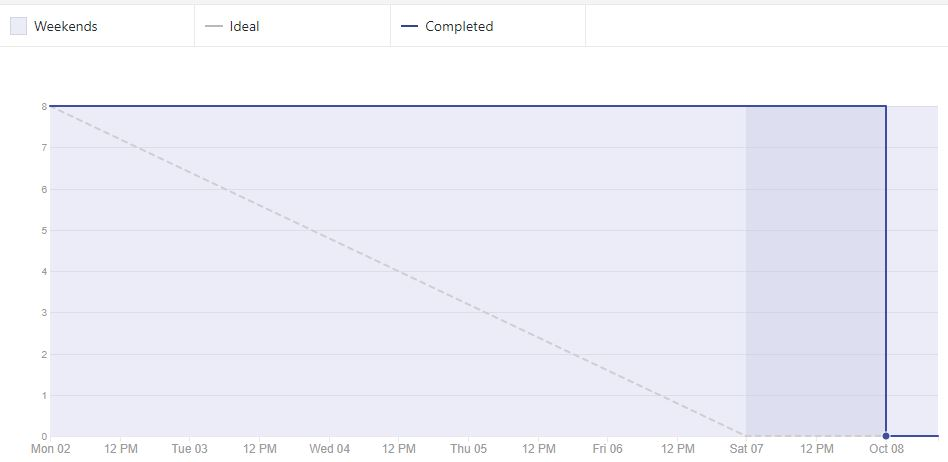
\includegraphics[width=1\textwidth]{imagenesAnexos/imagenesPlanificacion/sprint4}%
          \caption{Gráfico Burndown del sprint 4.}%
          \label{figSprint4}%
        \end{center}%
  	\end{center}%
\end{figure}%

Estos cuatro primeros sprints se dedicaron a estudiar las diferentes herramientas necesarias para implementar las propuestas del proyecto. La mayoría de estas herramientas eran desconocidas para mí por lo que me llevo un tiempo familiarizarme con ellas y empezar a implementar los diferentes programas.

En estos primeros sprints se consiguió crear en Android una aplicación que ejecutaba los modelos Mobilenet e Incpetion y en Java una aplicación que realizaba parte de las consultas necesarias a la DBpedia.

\subsection{Sprint 5}

Este sprint se desarrolló entre los días 11 y 18 de octubre de 2017. Se realizaron las siguientes tareas y objetivos:

\begin{itemize}
	\item Estudiar como implementar una base de datos SQL que funcione tanto en Android como en Windows.
	\item Implementar la base de datos en Windows para el programa de consultas a la web semántica.
	\item Implementar base de datos en la aplicación Android.
	\item Elegir una base de datos apropiada para los requisitos de la aplicación.
\end{itemize}

Para implementar la base de datos, se empezó estudiando e implementando una base de datos Microsoft JDBC en Windows con la intención de exportarla posteriormente a Android. Aunque se consiguió realizar esta parte, se decidió cambiar a una base de datos SQlite, ya que era mucho más ligera que la de Microsoft y más sencilla de usar para las necesidades básicas que tiene nuestra aplicación.

En esta semana se consiguió crear la base de datos y los métodos de acceso necesarios tanto en la aplicación de Eclipse como en la Android.

\begin{figure}[h]
    \begin{center}%
        \begin{center}%
          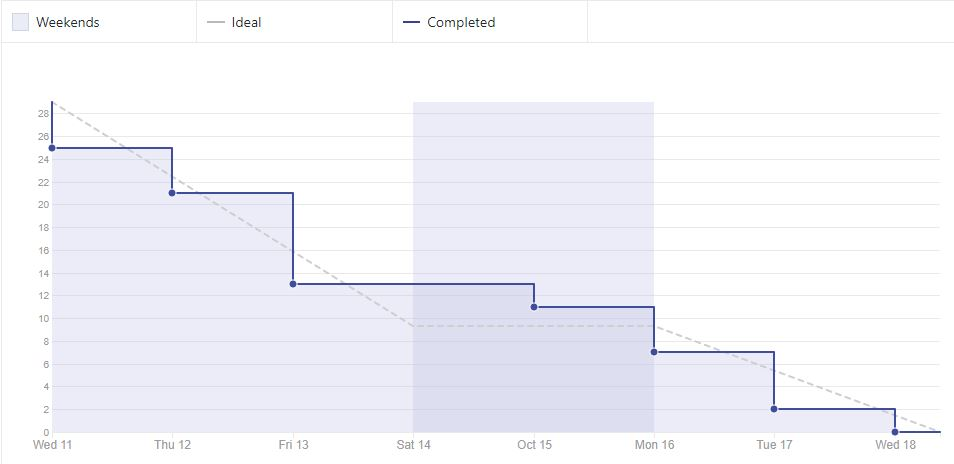
\includegraphics[width=0.9\textwidth]{imagenesAnexos/imagenesPlanificacion/sprint5}%
          \caption{Gráfico Burndown del sprint 5.}%
          \label{figSprint5}%
        \end{center}%
  	\end{center}%
\end{figure}%

\begin{figure}[h]
    \begin{center}%
        \begin{center}%
          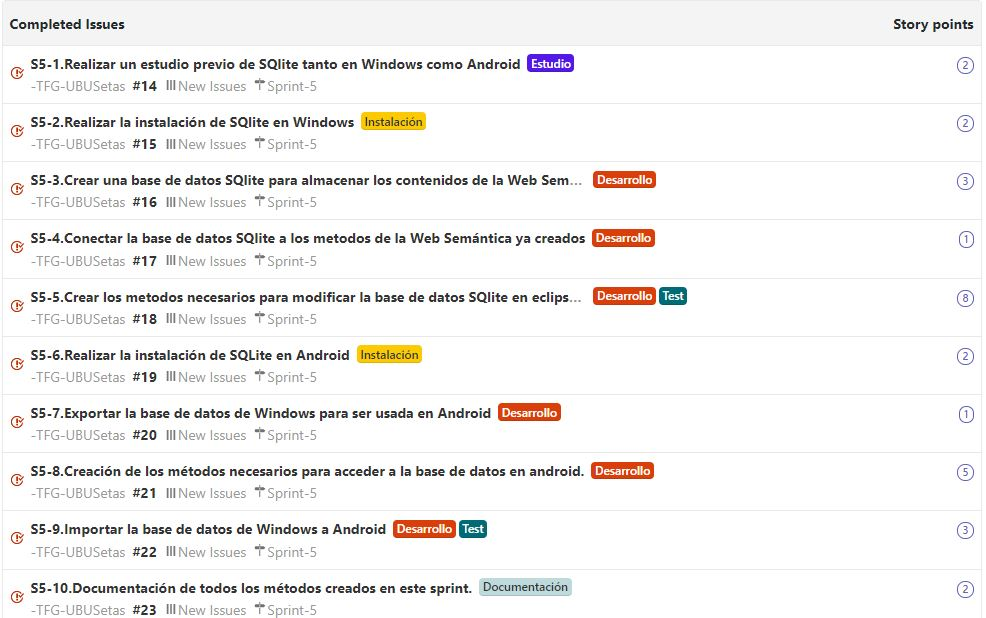
\includegraphics[width=0.9\textwidth]{imagenesAnexos/imagenesPlanificacion/tareas5}%
          \caption{Issues del sprint 5.}%
          \label{figTareas5}%
        \end{center}%
  	\end{center}%
\end{figure}%

\newpage

A partir de este sprint se empezó a utilizar de forma más correcta la Herramienta Zenhub y a mostrar de forma correcta las tareas desarrolladas en cada sprint.

\subsection{Sprint 6}

Este sprint se desarrolló entre los días 18 y 25 de octubre de 2017. Se realizaron las siguientes tareas y objetivos:

\begin{itemize}
	\item Crear la aplicación Java de acceso a la DBpedia a partir de las pruebas creadas.
	\item Crear la primera versión de la aplicación Android que muestre los resultados del clasificador.
	\item Crear un método en Java que traduzca textos de manera automática.
	\item Preparar la aplicación Android para mostrar los datos recibidos de la aplicación Java.
\end{itemize}

En esta semana se trabajó paralelamente tanto en la aplicación Android como en las consultas a la DBpedia. Se creó una versión Android que incorporaba las primeras actividades definidas en el prototipado. Se integró la información recogida por la aplicación Android en la base de datos de la aplicación Android.

Por último se creó un método Java que traducía realizando llamadas al traductor de Google, con el fin de entregar una aplicación internacionalizada tanto al español como el inglés.

\begin{figure}[h]
    \begin{center}%
        \begin{center}%
          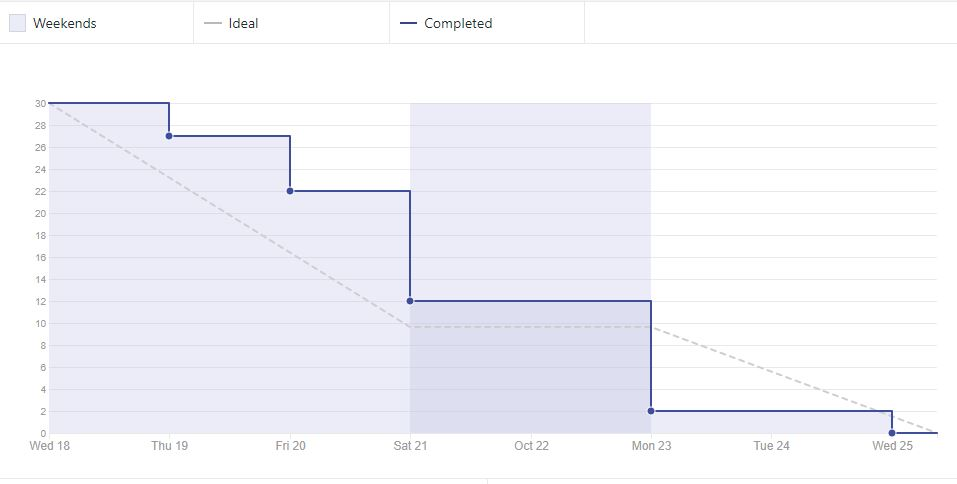
\includegraphics[width=0.9\textwidth]{imagenesAnexos/imagenesPlanificacion/sprint6}%
          \caption{Gráfico Burndown del sprint 6.}%
          \label{figSprint6}%
        \end{center}%
  	\end{center}%
\end{figure}%

\begin{figure}[h]
    \begin{center}%
        \begin{center}%
          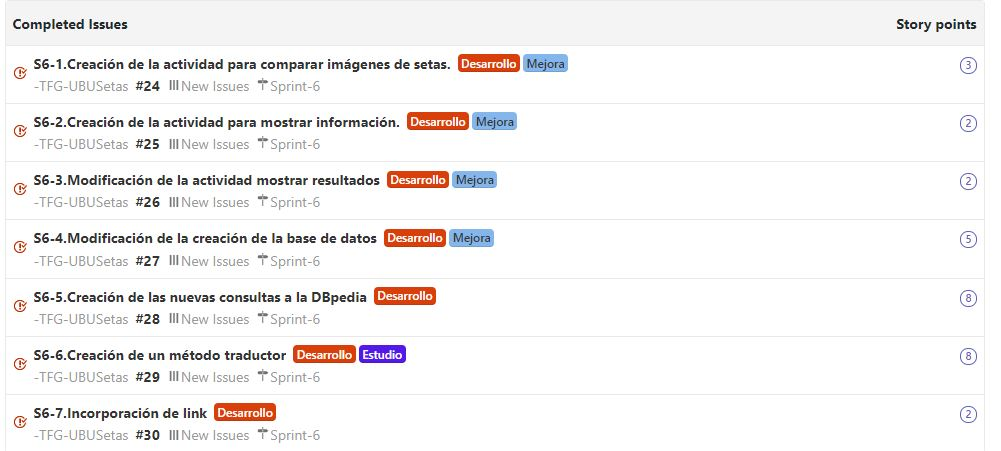
\includegraphics[width=0.9\textwidth]{imagenesAnexos/imagenesPlanificacion/tareas6}%
          \caption{Issues del sprint 6.}%
          \label{figTareas6}%
        \end{center}%
  	\end{center}%
\end{figure}%
\newpage

\subsection{Sprint 7}

Este sprint se desarrolló entre el día 25 de octubre y 1 de noviembre de 2017. Se realizaron las siguientes tareas y objetivos:

\begin{itemize}
	\item Estudiar como realizar Web Scraping en una página Web.
	\item Estudiar la herramienta \textit{Jaunt} para realizar Web Scraping en Java.
	\item Crear los métodos necesarios en el proyecto de Eclipse para extraer las claves dicotómicas de la página web \url{http://www.avelinosetas.info/claves.php}.
	\item Crear las actividades necesarias en la aplicación Android para mostrar las claves dicotómicas.
	\item Crear los métodos necesarios tanto en el proyecto Android y Eclipse para serializar las claves dicótomicas y transferirlas desde el proyecto de Eclipse a la aplicación Android.
\end{itemize}

En este sprint se encontró una página web con una clave dicotómica que contenía una gran cantidad de géneros de los clasificados por el clasificador, aunque no todos y mostraba claves de géneros para clasificar especies concretas de setas. Además la estructura html se repetía en todas las claves, lo que facilitó la aplicación de las técnicas de Web Scraping.

Se decidió serializar las claves dicotómicas en estructuras de datos Java para exportar de manera sencilla las claves a la aplicación Android, sin necesidad de tener que usar las base de datos SQlite.

\begin{figure}[h]
    \begin{center}%
        \begin{center}%
          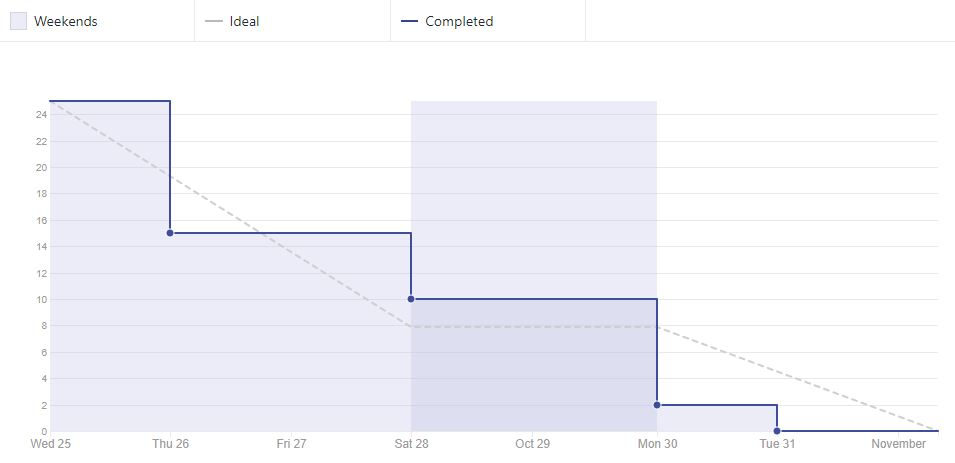
\includegraphics[width=0.9\textwidth]{imagenesAnexos/imagenesPlanificacion/sprint7}%
          \caption{Gráfico Burndown del sprint 7.}%
          \label{figSprint7}%
        \end{center}%
  	\end{center}%
\end{figure}%

\begin{figure}[h]
    \begin{center}%
        \begin{center}%
          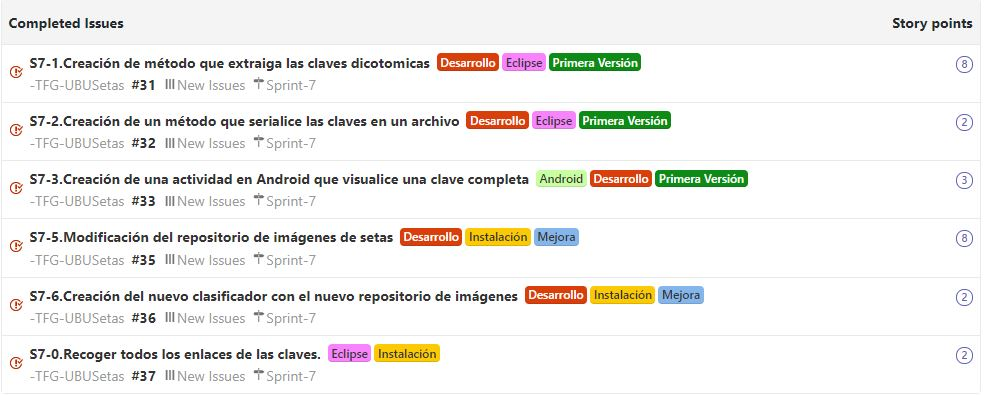
\includegraphics[width=0.9\textwidth]{imagenesAnexos/imagenesPlanificacion/tareas7}%
          \caption{Issues del sprint 7.}%
          \label{figTareas7}%
        \end{center}%
  	\end{center}%
\end{figure}%

\newpage

\subsection{Sprint 8}

Este sprint se desarrolló entre los días 2 y 8 de noviembre de 2017. Se realizaron las siguientes tareas y objetivos:

\begin{itemize}
	\item Extraer fotografías de las especies que se encuentran en la clave y no en el clasificador, con el fin de ampliar el número de especies recogidas por el clasificador.
	\item Reentrenar el clasificador con las nuevas imágenes recopiladas.
	\item Ajustar los métodos de la aplicación Java para que extraiga información de las nuevas especies.
	\item Añadir nueva información (género, comestibilidad y enlace) de las especies de setas para ser incorporada a la aplicación Android.
	\item Estudio de las directrices de \textit{material design} para implementar la interfaz de la aplicación Android.
	\item Estudiar el funcionamiento de la herramienta Latex para empezar la memoria de la documentación.
\end{itemize}

En esta semana se decidió ampliar el número de especies clasificadas por el clasificador aumentando el número hasta las 171 especies. El objetivo era que no hubiera especies contenidas en la clave dicotómica de géneros que si estuvieran en el clasificador, con el fin de aprovechar la clave conseguida.

Esto provocó la modificación de los métodos en ambas aplicaciones para extraer y manejar las nuevas especies incorporadas.

También se empezó a estudiar cómo realizar una mejor interfaz basándome en los consejos ofrecidos por \textit{material design}.

Se comenzó a estudiar la herramienta latex para empezar lo antes posible con la documentación del proyecto.

\begin{figure}[h]
    \begin{center}%
        \begin{center}%
          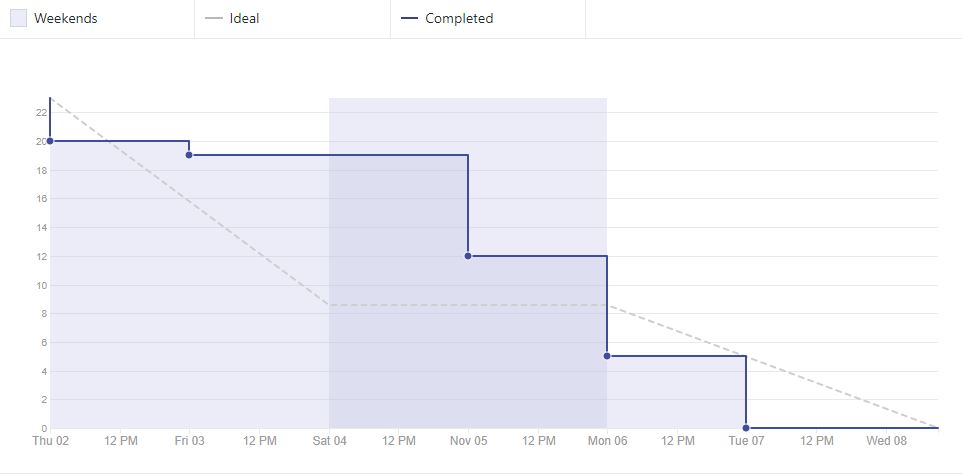
\includegraphics[width=0.9\textwidth]{imagenesAnexos/imagenesPlanificacion/sprint8}%
          \caption{Gráfico Burndown del sprint 8.}%
          \label{figSprint8}%
        \end{center}%
  	\end{center}%
\end{figure}%

\begin{figure}[h]
    \begin{center}%
        \begin{center}%
          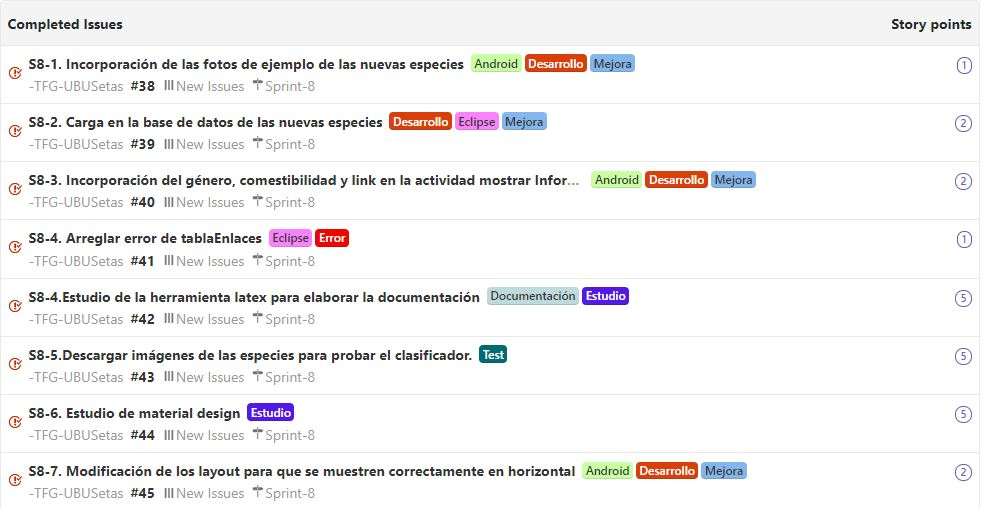
\includegraphics[width=0.9\textwidth]{imagenesAnexos/imagenesPlanificacion/tareas8}%
          \caption{Issues del sprint 8.}%
          \label{figTareas8}%
        \end{center}%
  	\end{center}%
\end{figure}%

\newpage

\subsection{Sprint 9}

Este sprint se desarrolló entre los días 8 y 15 de noviembre de 2017. Se realizaron las siguientes tareas y objetivos:

\begin{itemize}
	\item Escribir la introducción de la documentación.
	\item Escribir los objetivos del proyecto de la documentación.
	\item Escribir los conceptos teóricos de la documentación.
	\item Escribir las técnicas y herramientas de la documentación.
	\item Crear el prototipado para la interfaz de la aplicación Android.
\end{itemize}

Este sprint se dedicó a comenzar la documentación del proyecto y a crear un prototipado de la interfaz de la aplicación Android que sirviera de guía para construir la interfaz de la aplicación Android.

\begin{figure}[h]
    \begin{center}%
        \begin{center}%
          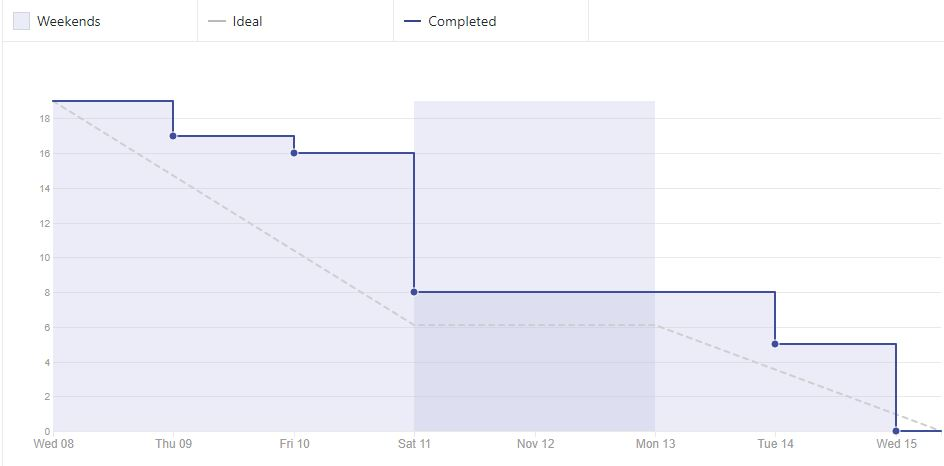
\includegraphics[width=0.9\textwidth]{imagenesAnexos/imagenesPlanificacion/sprint9}%
          \caption{Gráfico Burndown del sprint 9.}%
          \label{figSprint9}%
        \end{center}%
  	\end{center}%
\end{figure}%

\begin{figure}[h]
    \begin{center}%
        \begin{center}%
          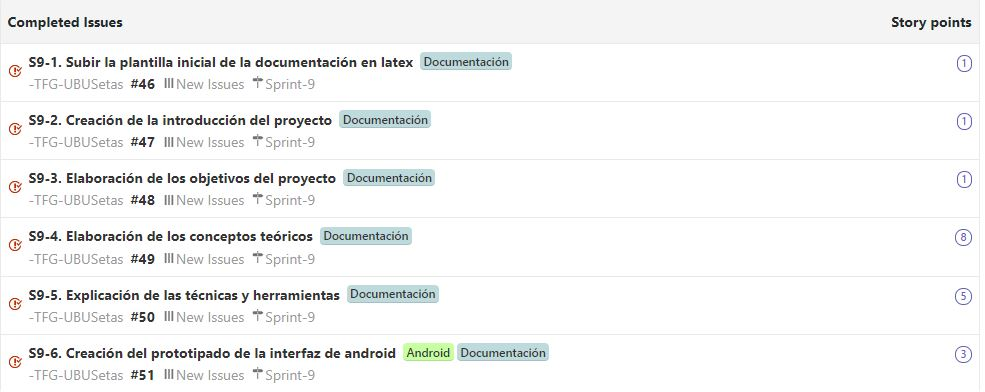
\includegraphics[width=0.9\textwidth]{imagenesAnexos/imagenesPlanificacion/tareas9}%
          \caption{Issues del sprint 9.}%
          \label{figTareas9}%
        \end{center}%
  	\end{center}%
\end{figure}%

\newpage

\subsection{Sprint 10}

Este sprint se desarrolló entre los días 15 y 22 de noviembre de 2017. Se realizaron las siguientes tareas y objetivos:

\begin{itemize}
	\item Construir la interfaz de las actividades creadas hasta este punto.
	\item Solucionar errores por los que las imágenes no se muestran correctamente en la aplicación Android.
	\item Seguir desarrollando la documentación.
	\item Creación de las actividades que muestran un listado de las especies y claves dicotómicas disponibles en la aplicación.
\end{itemize}

Esta semana se dedicó a seguir construyendo la aplicación Android, incorporando dos nuevas actividades que mostraran al usuario las claves dicotómicas e información de las diferentes especies disponibles.

Se corrigió un error por el que el tamaño de la foto insertada por el usuario afectaba en los resultados ofrecidos por el clasificador, ya que se debían proporcionar imágenes escaladas a 224x224 pixeles de tamaño al clasificador para un correcto funcionamiento.

Se revisó la documentación creada en el sprint anterior.

\begin{figure}[h]
    \begin{center}%
        \begin{center}%
          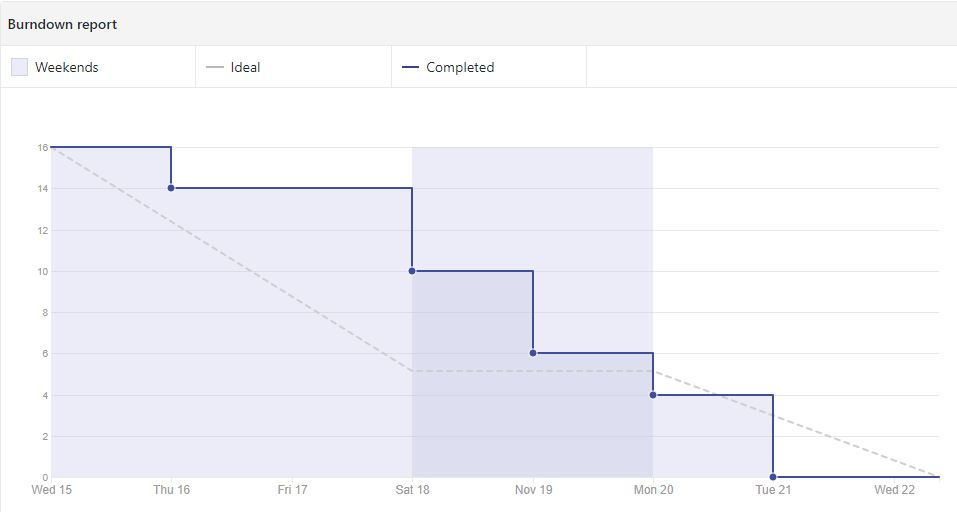
\includegraphics[width=0.9\textwidth]{imagenesAnexos/imagenesPlanificacion/sprint10}%
          \caption{Gráfico Burndown del sprint 10.}%
          \label{figSprint10}%
        \end{center}%
  	\end{center}%
\end{figure}%

\begin{figure}[h]
    \begin{center}%
        \begin{center}%
          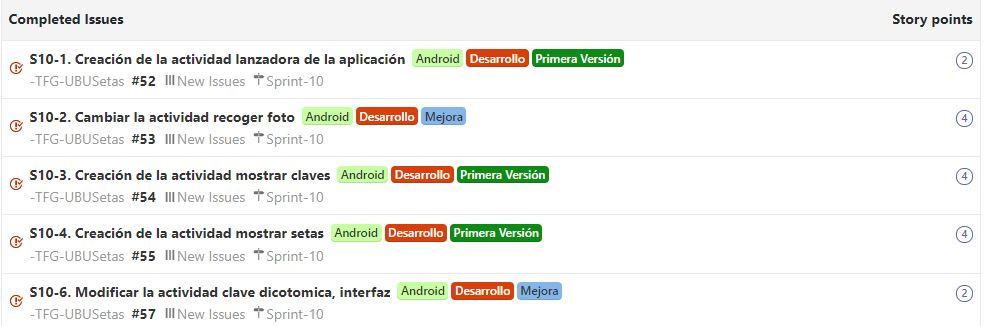
\includegraphics[width=0.9\textwidth]{imagenesAnexos/imagenesPlanificacion/tareas10}%
          \caption{Issues del sprint 10.}%
          \label{figTareas10}%
        \end{center}%
  	\end{center}%
\end{figure}%

\newpage

\subsection{Sprint 11}

Este sprint se desarrolló entre los días 22 y 30 de noviembre de 2017. Se realizaron las siguientes tareas y objetivos:

\begin{itemize}
	\item Seguir desarrollando la interfaz Android.
	\item Crear una actividad que pida al usuario elegir sobre que géneros, de los clasificados, desea aplicar la clave dicotómica para concretar las preguntas realizadas en esos géneros.
	\item Seguir desarrollando la documentación.
	\item Corregir pequeños errores de funcionamiento de la interfaz.
	\item Generar la primera \textit{release} del proyecto.
\end{itemize}

En este sprint se siguió implementado la aplicación Android añadiendo nuevas funcionalidades, como el filtrado de géneros de la clave dicotómica. Así como corregir pequeños errores que se encontraron en la interfaz.

Tras realizar estas tareas se lanzó la primera \textit{release} del proyecto.

Se terminaron los puntos de la memoria que no habían sido completados todavía.

\begin{figure}[h]
    \begin{center}%
        \begin{center}%
          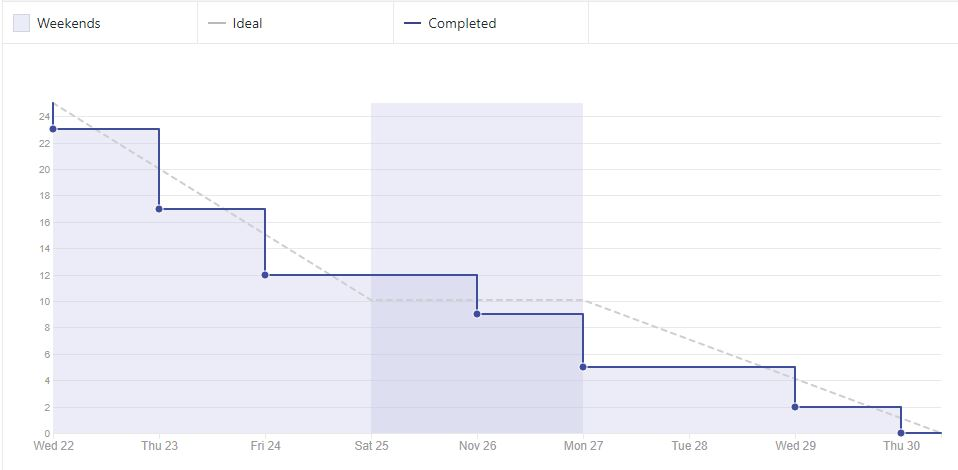
\includegraphics[width=0.9\textwidth]{imagenesAnexos/imagenesPlanificacion/sprint11}%
          \caption{Gráfico Burndown del sprint 11.}%
          \label{figSprint11}%
        \end{center}%
  	\end{center}%
\end{figure}%

\begin{figure}[h]
    \begin{center}%
        \begin{center}%
          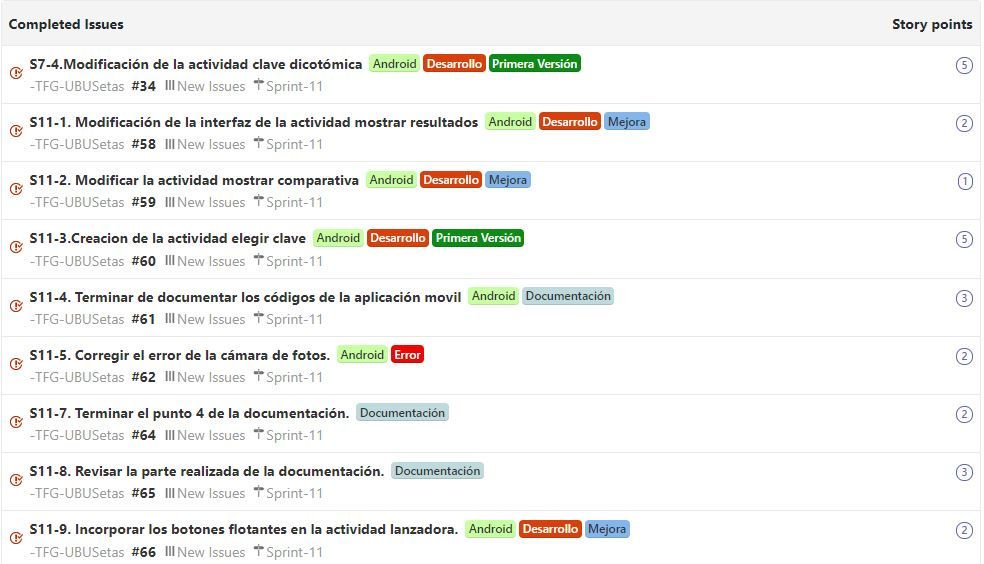
\includegraphics[width=0.9\textwidth]{imagenesAnexos/imagenesPlanificacion/tareas11}%
          \caption{Issues del sprint 11.}%
          \label{figTareas11}%
        \end{center}%
  	\end{center}%
\end{figure}%

\newpage

\subsection{Sprint 12}

Este sprint se desarrolló entre el día 30 de noviembre al 7 de diciembre de 2017. Se realizaron las siguientes tareas y objetivos:

\begin{itemize}
	\item Traducir todos los textos de la aplicación, claves e información al inglés.
	\item Internacionalizar la aplicación permitiendo que el usuario pueda elegir entre el español y el inglés, pudiendo cambiar en cualquier momento.
	\item Modificar el proyecto de Eclipse para que se traduzcan automáticamente todas las claves dicotómicas.
	\item Incorporar botones que muestren ayuda dentro de la aplicación al usuario en todas las actividades.
	\item Corregir errores en la rotación de pantalla de la aplicación Android.
\end{itemize}

Esta semana se dedicó a traducir todos los textos de la aplicación Android al inglés, lo que provocó que se necesitara modificar el método extractor de claves dicotómicas del proyecto de Eclipse para que a la vez que extrajera las claves, las tradujera al inglés.

Se añadieron páginas de ayuda de usuario, dentro de la aplicación Android, para explicar la funcionalidad de cada elemento que se muestra al usuario en pantalla. Para acceder a ella, el usuario solo debe pulsar el botón de ayuda, o el item de ayuda disponible en el menú de la aplicación.

\begin{figure}[h]
    \begin{center}%
        \begin{center}%
          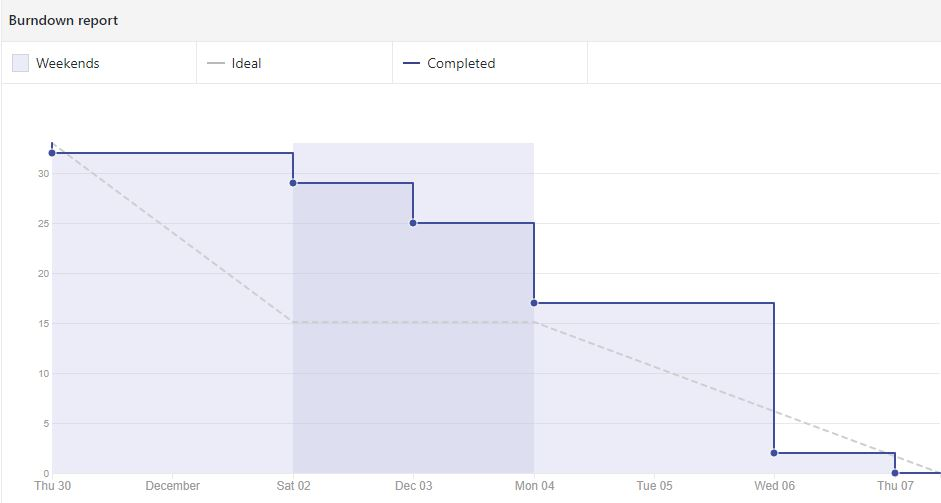
\includegraphics[width=0.9\textwidth]{imagenesAnexos/imagenesPlanificacion/sprint12}%
          \caption{Gráfico Burndown del sprint 12.}%
          \label{figSprint12}%
        \end{center}%
  	\end{center}%
\end{figure}%

\begin{figure}[h]
    \begin{center}%
        \begin{center}%
          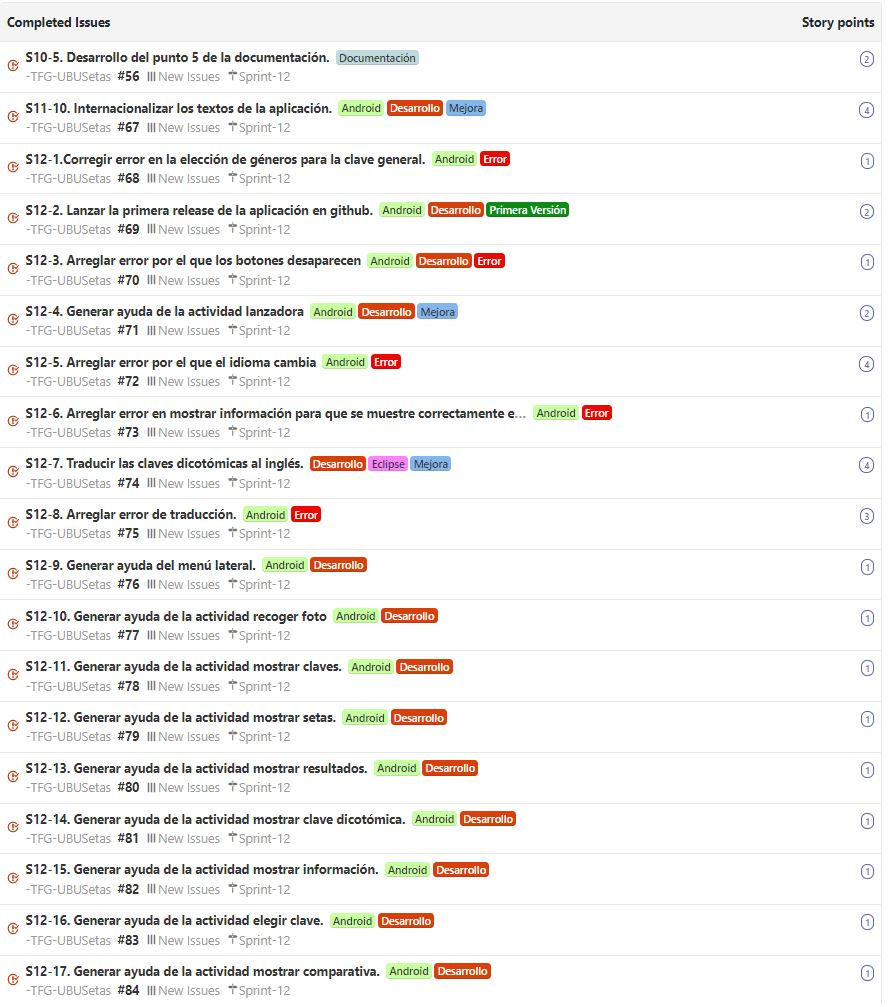
\includegraphics[width=0.9\textwidth]{imagenesAnexos/imagenesPlanificacion/tareas12}%
          \caption{Issues del sprint 12.}%
          \label{figTareas12}%
        \end{center}%
  	\end{center}%
\end{figure}%

\newpage

\subsection{Sprint 13}

Este sprint se desarrolló entre los días 7 y 14 de diciembre de 2017. Se realizaron las siguientes tareas y objetivos:

\begin{itemize}
	\item Estudiar la herramienta\textit{Roboelectric} para realizar los test unitarios en Android Studio.
	\item Estudiar las herramientas \textit{Espresso} y \textit{UIautomator} para realizar las pruebas de integración en Android Studio. 
	\item Realizar los primeros test unitarios de la aplicación.
	\item Incorporar botones que muestren ayuda dentro de la aplicación al usuario en todas las actividades.
	\item Escribir el punto de \textit{Aspectos relevantes del desarrollo
del proyecto} de la documentación.
	\item Escribir el punto de \textit{Trabajos relacioandos} de la documentación.
	\item Escribir el punto de \textit{Conclusiones y Líneas de trabajo
futuras} de la documentación.
\end{itemize}

Este sprint se dedicó a estudiar cómo realizar los test unitarios y de integración a la aplicación Android.

Se elaborarón los primeros test unitarios y se siguió avanzando en el desarrollo de la documentación.

\begin{figure}[h]
    \begin{center}%
        \begin{center}%
          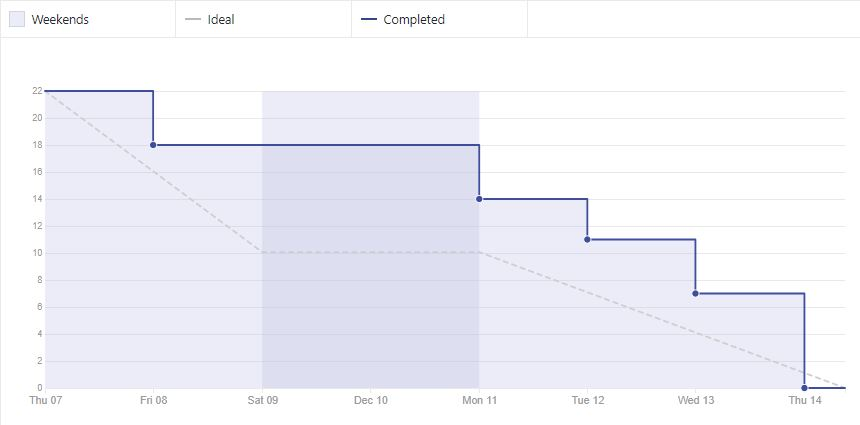
\includegraphics[width=0.9\textwidth]{imagenesAnexos/imagenesPlanificacion/sprint13}%
          \caption{Gráfico Burndown del sprint 13.}%
          \label{figSprint13}%
        \end{center}%
  	\end{center}%
\end{figure}%

\begin{figure}[h]
    \begin{center}%
        \begin{center}%
          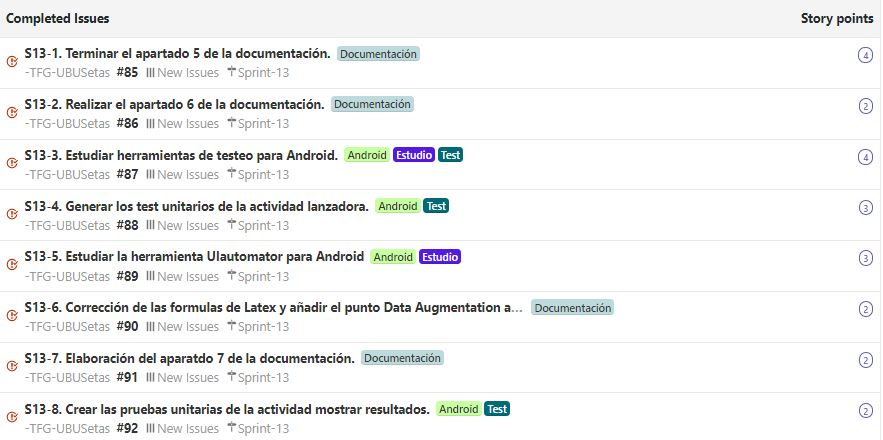
\includegraphics[width=0.9\textwidth]{imagenesAnexos/imagenesPlanificacion/tareas13}%
          \caption{Issues del sprint 13.}%
          \label{figTareas13}%
        \end{center}%
  	\end{center}%
\end{figure}%

\newpage

\subsection{Sprint 14}

Este sprint se desarrolló entre los días 14 y 21 de diciembre de 2017. Se realizaron las siguientes tareas y objetivos:

\begin{itemize}
	\item Realizar los test unitarios de todas las actividades de la aplicación Android.
	\item Realizar todos los test de integración de la aplicación Android.
	\item Estudiar la herramienta \textit{monkeyrunner} para crear test de rendimiento.
\end{itemize}

Este sprint se dedicó a realizar pruebas unitarias y de integración sobre todas las actividades de la aplicación Android.

También se estudió la herramienta \textit{monkeyrunner} para crear una serie de eventos aleatorios sobre la aplicación y comprobar la robustez de esta.
\newpage
\begin{figure}[ht]
    \begin{center}%
        \begin{center}%
          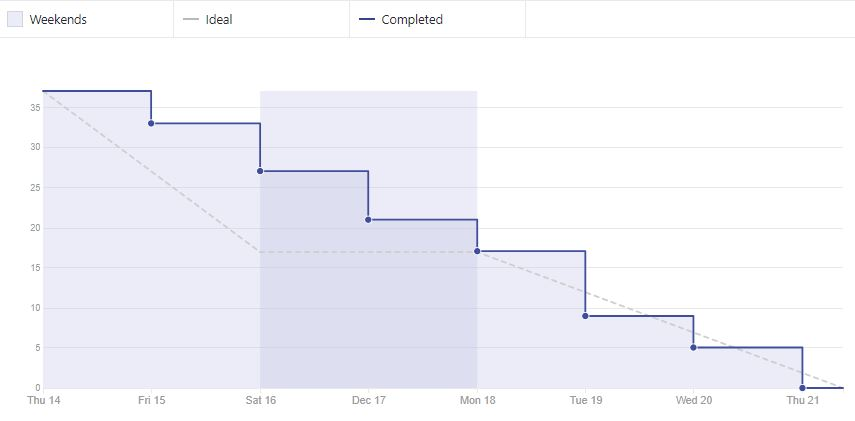
\includegraphics[width=0.9\textwidth]{imagenesAnexos/imagenesPlanificacion/sprint14}%
          \caption{Gráfico Burndown del sprint 14.}%
          \label{figSprint14}%
        \end{center}%
  	\end{center}%
\end{figure}%
\newpage
\begin{figure}[h]
    \begin{center}%
        \begin{center}%
          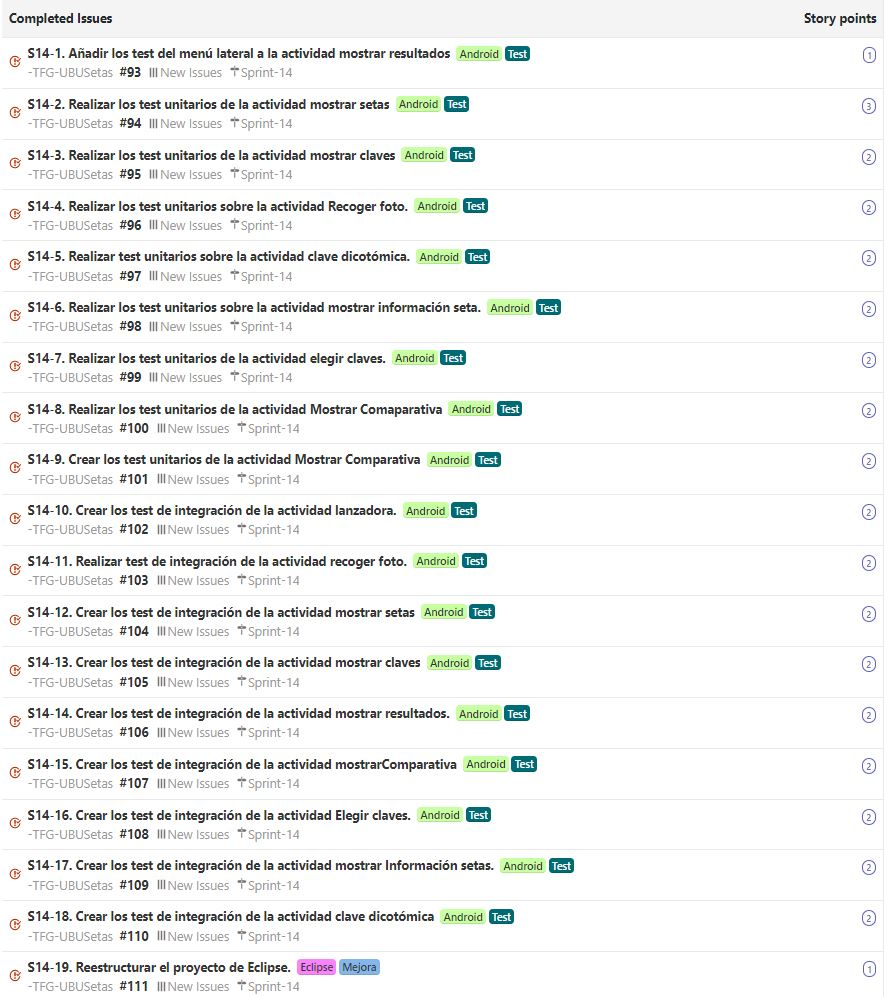
\includegraphics[width=0.9\textwidth]{imagenesAnexos/imagenesPlanificacion/tareas14}%
          \caption{Issues del sprint 14.}%
          \label{figTareas14}%
        \end{center}%
  	\end{center}%
\end{figure}%

\newpage
\section{Estudio de viabilidad}

En este apartado se va a hacer un estudio sobre la viabilidad económica y legal del proyecto.

\subsection{Viabilidad económica}

En esta sección se va a hacer una aproximación de los costes que supondría para una empresa el desarrollo de este proyecto

\subsubsection{Coste del personal}

La realización de este proyecto ha necesitado de cuatro meses en los que estaría empleado un desarrollador. Vamos a suponer que este desarrollador tiene un salario bruto de 1500 euros.

Ahora habrá que calcular los gastos de seguridad social\footnote{\url{http://www.seg-social.es/Internet_1/Trabajadores/CotizacionRecaudaci10777/Basesytiposdecotiza36537/index.htm}}, tanto por parte de la empresa como del trabajador:

Por parte de la empresa:

\begin{itemize}
	\item Contingencias comunes: 23,6\%
	\item Desempleo: 5,5\%
	\item Fogasa: 0,2\%
	\item Formación profesional: 0,6\%
\end{itemize}

Por parte del trabajador:

\begin{itemize}
	\item Contingencias comunes: 4,7\%
	\item Desempleo: 1,55\%
	\item Formación profesional: 0,1\%
\end{itemize}

Hacen un total del 29,9\% por parte de la empresa y el 6,35\% por parte del trabajador.

\tablaSmallSinColores{Costes de personal}{p{6.4cm} p{2.15cm} p{8cm}}{costespersonales}{
  \multicolumn{1}{p{4.5cm}}{\textbf{Concepto}} & \textbf{Coste{}}\\
 }
 {
  Salario mensual neto  & \multicolumn{1}{r}{1.224,75}\\
  Retención IRPF (12\%) & \multicolumn{1}{r}{180}\\
  Seguridad social (Empleado) (6,35\%) & \multicolumn{1}{r}{95,25}\\
  Salario mensual bruto  & \multicolumn{1}{r}{1.500}\\\hline
  Salario total (4 meses)  & \multicolumn{1}{r}{6.000}\\\hline
  Seguridad social (Empresa) (29,9\%) & \multicolumn{1}{r}{448,5}\\\hline
  Coste total mensual de la empresa & \multicolumn{1}{r}{1794}\\\hline
  }
  
\subsubsection{Coste informáticos}

A nivel de software no hay gastos ya que todas las librerías son gratuitas y no necesitamos pagar ningún servidor para mantener nuestra aplicación. A nivel hardware solamente se ha usado mi ordenador portátil por valor de 700 euros. La amortización es de 5 años y se ha usado 4 meses por lo que el coste es el siguiente:

\[(700euros/(12 meses * 4 periodos))* 4 meses=58,33euros\]

\subsubsection{Coste total}

En la siguiente tabla se recoge el coste total del proyecto.

 \tablaSmallSinColores{Costes totales}{p{6.4cm} p{2.15cm} p{8cm}}{costestotales}{
  \multicolumn{1}{p{4.5cm}}{\textbf{Concepto}} & \textbf{Coste {}}\\
 }
 {
  Salario empleado  & \multicolumn{1}{r}{6000}\\
  Seguridad social & \multicolumn{1}{r}{1794}\\
  Costes hardware(6,35\%) & \multicolumn{1}{r}{58,33}\\
  Total & \multicolumn{1}{r}{7852,33}\\\hline
  }

\subsection{Viabilidad legal}


En esta sección se recogerá una tabla con las distintas licencias de las librerías usadas en el proyecto.

\tablaSmallSinColores{Licencias}{p{6.4cm} p{2.15cm} p{8cm}}{licencias}{
  \multicolumn{1}{p{4.5cm}}{\textbf{Librería}} & \textbf{Licencia}\\
 }
 {
  Tensorflow & \multicolumn{1}{r}{Apache 2.0 opensource license}\\
  Apache jena & \multicolumn{1}{r}{Apache License 2.0}\\
  Json & \multicolumn{1}{r}{Libre}\\
  Jaunt & \multicolumn{1}{r}{Libre mensualmente}\\
  SQlite & \multicolumn{1}{r}{Libre}\\
  }
  
Respecto a la licencia de Jaunt, hay que mencionar que es una librería que hay que descargar cada mes, ya que se actualiza y deja de funcionar pasado ese tiempo.

